The system includes a web-based application for visualizing maps and paths of the agents. The application is designed to be accessible via the internet, providing a user-friendly interface for monitoring the agents' movements. The web application will connect to the system's data source to retrieve live data in real-time. This allows for real-time monitoring of the agent's actions and provides a powerful tool for understanding the behavior of the system. A mockup of the visualization is presented in Figure \ref{fig:vis_mock}, which provides an example of the type of information that will be presented in the web application. 

\begin{figure}[H]
    \centering
    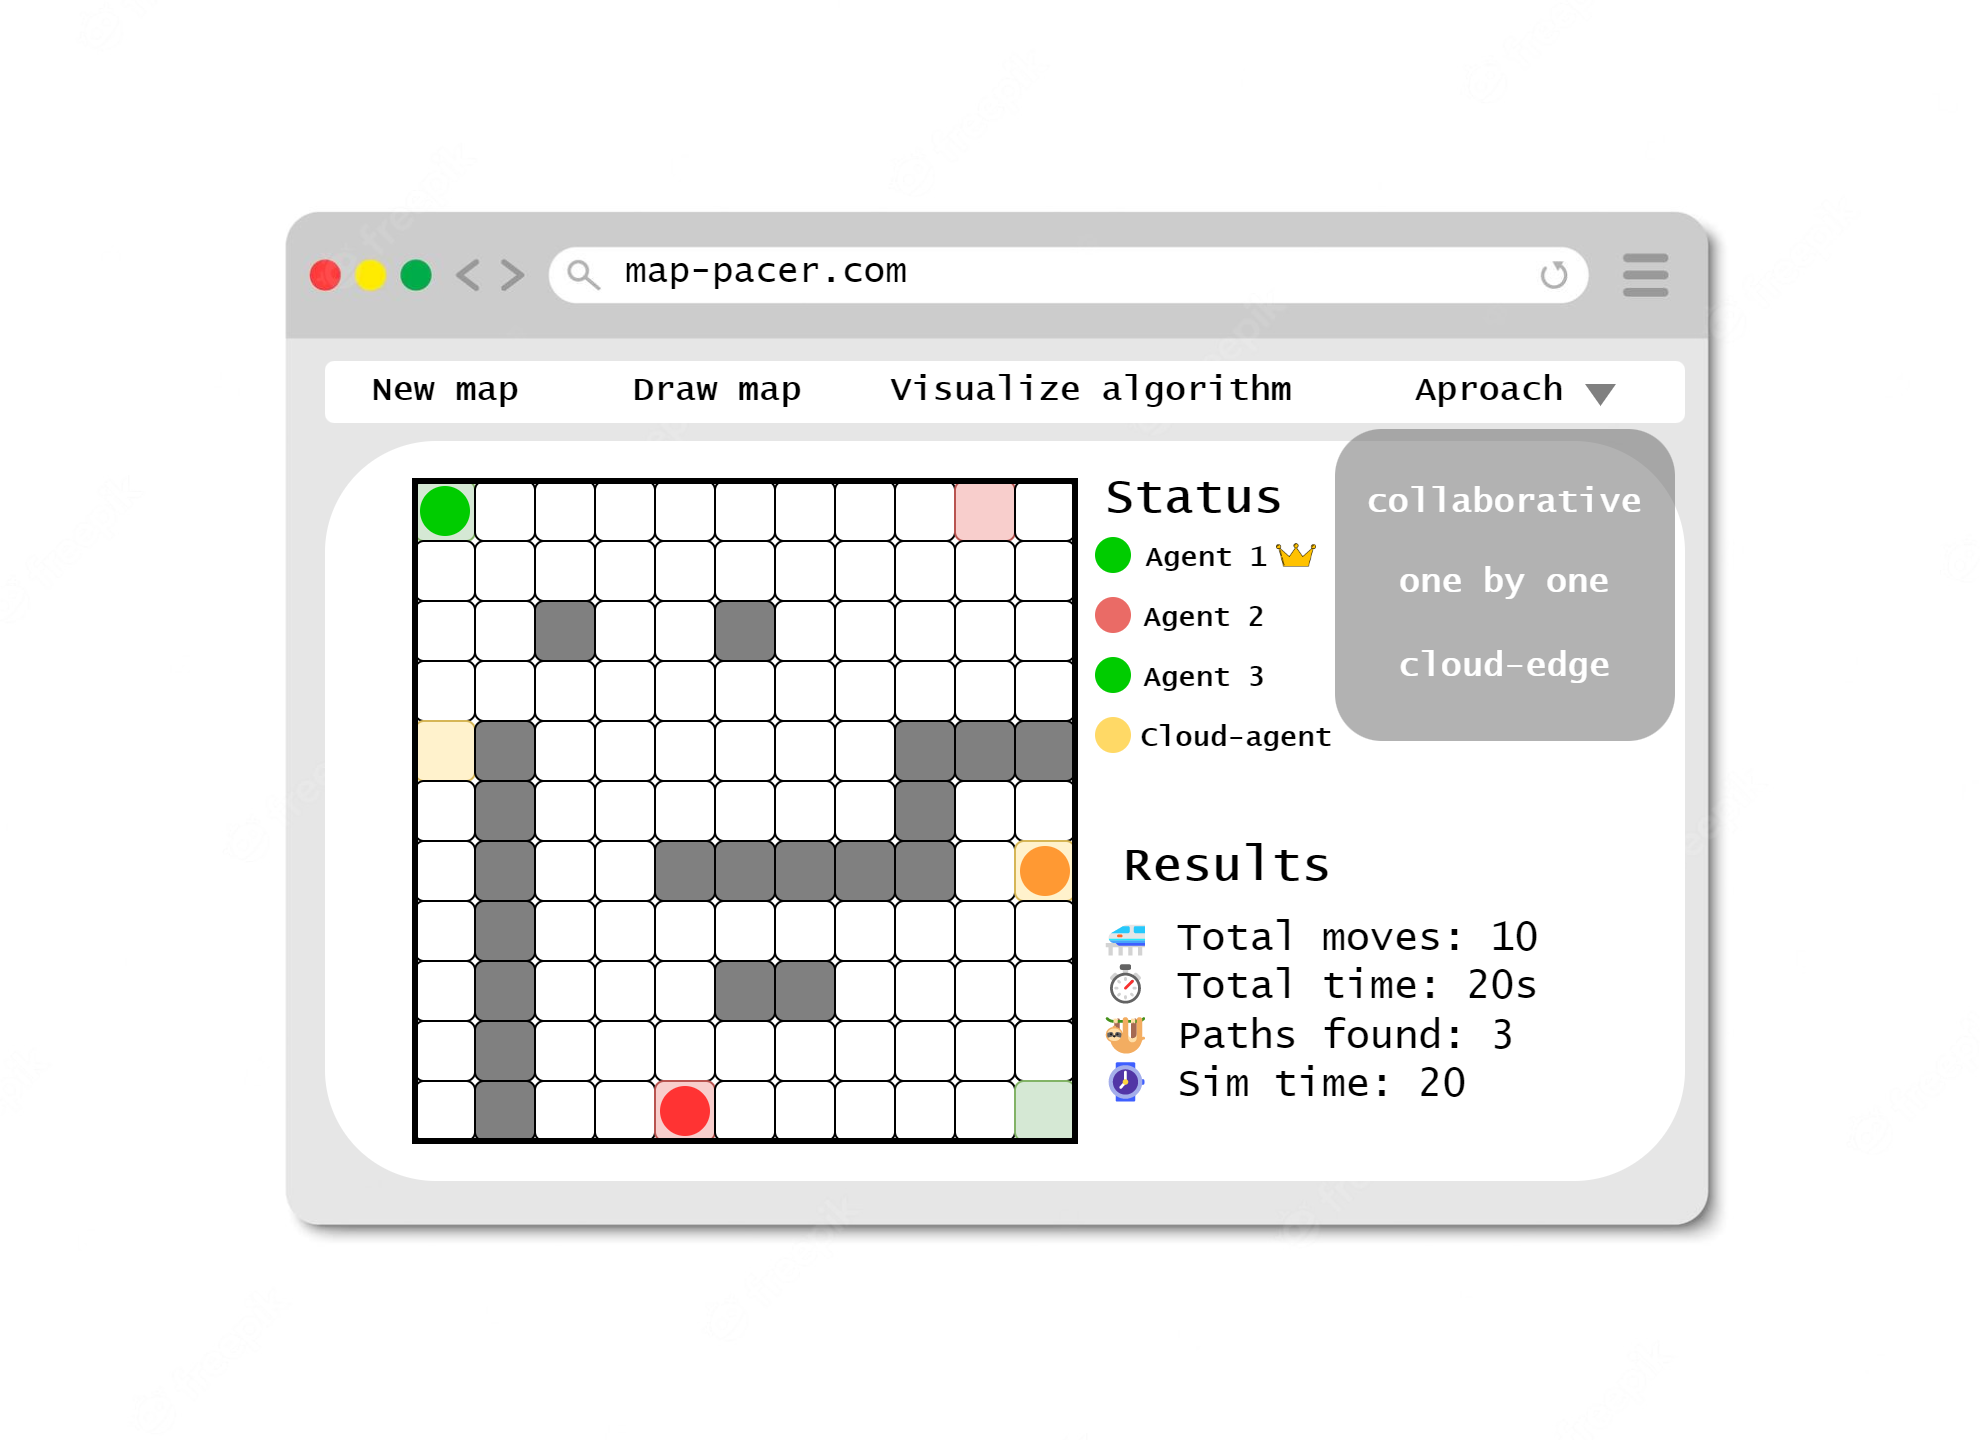
\includegraphics[width=\textwidth]{pictures/frontenf_mock.png}
    \caption{ Mock of the visualization }
    \label{fig:vis_mock}
\end{figure}

The graphical interface of the system will be centered around a grid map, which clearly displays the positions and goals of all the agents as colored dots. The status of the agents, the current leader, and other relevant information about the outcome of the algorithm will be displayed alongside the map.

Through a web application, the user will be able to:
\begin{itemize}
\itemsep0em 
    \item Generate new map (random or predefined map)
    \item Create new map
    \item Select algorithm
    \item Visualize algorithm
\end{itemize}
Additional features may include:
\begin{itemize}
\itemsep0em 
    \item Access map creator, to specify own map.
    \item Choose among different systems (multi-tenancy).
    \item Reply visualization.
\end{itemize}